\section{Mesh-Aligned Pseudo-Labeling}
\label{sec:mapl}

\begin{figure}[t]
    \centering
    \begin{tikzpicture}[font=\scriptsize, node distance=2.5mm and 3mm,
        box/.style={draw, rounded corners=1pt, align=center, inner sep=2pt, minimum height=5mm, fill=white},
        data/.style={box, fill=black!5}, model/.style={box, fill=blue!8}, rend/.style={box, fill=orange!12},
        arr/.style={-{Latex[length=1.5mm]}, thick}]
        \node[data, text width=31mm] (lab) {$\Kreal$ labeled frames per object (depth, pose)};
        \node[data, text width=26mm, right=of lab] (mesh) {object meshes};
        \node[model, text width=31mm, below=of lab] (f0) {teacher $f_0$ ($\Kreal$-shot model)};
        \node[rend, text width=26mm, below=of mesh] (al) {aligner $A$: (frame, mesh depth at pose) $\to$ pose correction};
        \node[data, text width=31mm, below=4.5mm of f0] (unl) {unlabeled frames $U$};
        \node[box, text width=26mm, right=of unl] (rc) {\textbf{align}: iterate $A$ from the teacher pose};
        \node[model, text width=31mm, below=of unl] (f1) {student $f_1$: $\Kreal$ labeled + aligned $U$};
        \node[box, text width=26mm, below=of rc] (lbl) {\textbf{label}: mesh depth, normals and pose at the aligned pose};
        \draw[arr] (lab) -- (f0); \draw[arr] (lab) -- (al); \draw[arr] (mesh) -- (al);
        \draw[arr] (f0) -- node[left, xshift=-1pt] {pose} (unl); \draw[arr] (unl) -- (rc); \draw[arr] (al) -- (rc);
        \draw[arr] (rc) -- (lbl); \draw[arr] (lbl) -- (f1);
    \end{tikzpicture}
    \caption{\textbf{Mesh-aligned pseudo-labeling.} The $\Kreal$-shot teacher proposes a pose for every unlabeled frame. An aligner trained on the same $\Kreal$ labeled frames iteratively corrects that pose until the object mesh matches the frame; the mesh at the aligned pose, not the teacher's prediction, labels the frame for the student.}
    \label{fig:mapl}
\end{figure}

\begin{figure}[t]
    \centering
    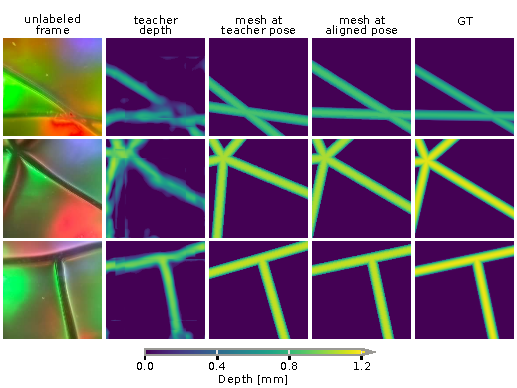
\includegraphics[width=\columnwidth]{figures/fig_align.pdf}
    \caption{\textbf{Labels of unlabeled frames} ($\Kreal=25$; each object's median-quality frame). The teacher's depth is blurred and its pose is off by several degrees; after alignment the mesh label is close to the withheld reference.}
    \label{fig:align}
\end{figure}

\noindent\textbf{Idea.} Let $d(M,q)$ be the depth map of mesh $M$ at contact state $q=(\theta,x,y,z)$ (planar pose and indentation). The reference label of a real frame $I$ of object $M$ is $d(M,q^\ast)$ for the pose $q^\ast$ at which it was captured, so labeling an unlabeled frame is a pose-estimation problem with only four unknowns, and its solution yields depth, normals and pose at once. A $\Kreal$-shot model estimates $q$ only to a few degrees and its dense output is blurred (Fig.~\ref{fig:align}); with the true pose, in contrast, the mesh label is essentially exact (contact IoU $0.95$ against the reference). MAPL closes this gap with a learned refinement.

\noindent\textbf{Residual aligner.} The aligner $A$ is a ResNet-18 (ImageNet-initialized) that takes the real frame and, as a fourth channel, the mesh depth at a candidate pose, and regresses the correction that brings the candidate onto the frame:
\begin{equation}
    A\big(I,\; d(M,q)\big) \;\approx\; q^\ast - q .
\end{equation}
It needs no label beyond the $\Kreal$ frames, because each labeled frame provides unlimited training pairs: we perturb its true pose by up to $\pm8^\circ$, $\pm1.5\,$mm in the plane and $\pm0.15\,$mm of indentation (half of the samples at $0.3\times$ that range, for fine corrections), render the mesh depth at the perturbed pose, and regress the perturbation with a smooth-L1 loss (8k steps, batch 64, AdamW, $3\times10^{-4}$). This is render-and-compare pose refinement~\cite{li2018deepim} with the mesh depth as the ``render'': no photorealistic renderer is involved.

\noindent\textbf{Labeling.} For every unlabeled training frame the teacher $f_0$ (the model trained on the $\Kreal$ labeled frames and GAN-$\Kreal$ data) predicts a pose; the indentation is initialized with the maximum of its predicted depth. The aligner is applied six times, $q\leftarrow q+A(I,d(M,q))$, and the frame receives $d(M,q)$, its normals and $q$ as labels. Every frame is used; no confidence filtering is needed (Sec.~\ref{sec:ablation}). The object of each frame is assumed known, as it is when a user collects frames object by object.

\noindent\textbf{Student.} The student $f_1$ is trained like any other model in this paper on the $\Kreal$ labeled frames, the aligned frames and synthetic frames, with full depth, normal and pose supervision. Following the $\Kreal$-shot rule, the synthetic frames come from the learned renderer retrained on the $\Kreal$ true plus the aligned (depth, image) pairs, which also makes it the most faithful leakage-free renderer of our study (contact-region image error $-13$ to $-19\%$ at every $\Kreal$); the student's accuracy, however, does not depend on this choice (Table~\ref{tab:abl}).

\noindent\textbf{Test-time alignment.} Planar pose is defined with respect to a known object, so the same aligner can also refine the pose a model predicts on a \emph{test} frame (Sec.~\ref{sec:tta}).

\noindent\textbf{Cost and scope.} MAPL adds no labels and leaves the downstream architecture unchanged; it uses the unlabeled frames and the meshes that simulation already requires. Validation and test frames are never pseudo-labeled and never seen by the aligner.
